
\chapter{Le théorème des cinq couleurs}\label{c.five}

%%%%%%%%%%%%%%%%%%%%%%%%%%%%%%%%%%%%%%%%%%%%%%%%%%%%%%%%%%%%%%%



Les cartes utilisent des couleurs pour distinguer une région d'une autre en veillant à ce que les régions adjacentes soient coloriées avec des couleurs différentes. En 1852, Francis Guthrie a remarqué qu'une carte des comtés d'Angleterre pouvait être coloriée en utilisant seulement quatre couleurs. L'affirmation selon laquelle quatre couleurs suffisent à colorier toute carte plane est appelée le théorème des quatre couleurs et n'a été démontrée qu'en 1976 par Kenneth Appel et Wolfgang Haken. Ils ont utilisé des arguments mathématiques sophistiqués pour montrer que s'il existe un contre-exemple (une carte nécessitant plus de quatre couleurs), il doit être associé à une configuration parmi $1834$. Ils ont ensuite utilisé un ordinateur pour examiner ces configurations.

Si le théorème des quatre couleurs est extrêmement difficile à démontrer, les démonstrations des théorèmes des cinq et six couleurs sont relativement simples (sect.~\ref{s.six-color} et \ref{s.five-color}). Pour démontrer ces théorèmes, nous définissons les cartes et les graphes planaires (sect.~\ref{s.planar}), démontrons la formule d'Euler (sect.~\ref{s.euler}) et montrons qu'un graphe planaire doit avoir un sommet dont le degré est inférieur ou égal à cinq. Dans la section~\ref{s.nonplanar}, la formule d'Euler est utilisée pour démontrer que deux graphes ne sont pas planaires.

En 1879, Alfred B. Kempe a publié une démonstration du théorème des quatre couleurs, mais  Percy J. Heawood a montré en 1890 que cette démonstration n'était pas correcte. Dans la section~\ref{s.kempe}, nous présentons la démonstration erronée de Kempe et la démonstration par Heawood qu'elle n'est pas correcte.

\section{Cartes  et graphes planaires}\label{s.planar}

\begin{definition}
Une \emph{carte planaire} est un ensemble de régions du plan séparées par des frontières. Un \emph{coloriage} d'une carte est l'attribution d'une couleur à chaque région, de sorte que les régions partageant une frontière reçoivent des couleurs différentes.
\end{definition}

La figure~\ref{f.five-planar-map-five} montre une carte planaire avec dix régions et cinq couleurs.
La figure~\ref{f.five-planar-map-four} montre la même carte coloriée avec quatre couleurs.

\vspace{0.4cm}

\begin{minipage}{0.42\textwidth}
\centering    
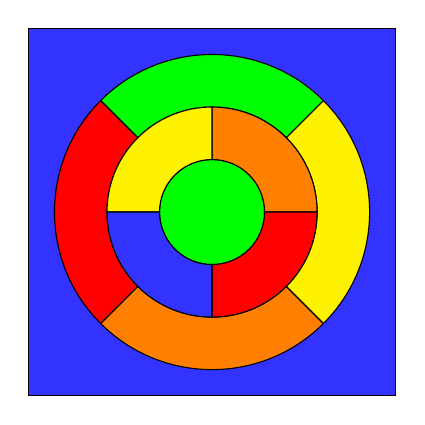
\begin{tikzpicture}[scale=.667]
\draw[fill=blue!80] (-3.5,-3.5) rectangle +(7,7);

\draw[fill=green] (0:1) 
  arc [start angle=0,  end angle=360, radius=1];

\draw[fill=green] (45:2) --
      (45:3)  arc[start angle=45,  end angle=135, radius=3] --
      (135:2) arc[start angle=135, end angle=45,  radius=2];
\draw[fill=orange] (-45:2) --
      (-45:3)  arc[start angle=-45,  end angle=-135, radius=3] --
      (-135:2) arc[start angle=-135, end angle=-45,  radius=2];
\draw[fill=yellow] (45:2) --
      (45:3)  arc[start angle=45,  end angle=-45, radius=3] --
      (-45:2) arc[start angle=-45, end angle=45,  radius=2];
\draw[fill=red] (135:2) --
      (135:3)  arc[start angle=135,  end angle=225, radius=3] --
      (225:2) arc[start angle=225, end angle=135,  radius=2];

\draw[fill=orange] (0:1) --
      (0:2)  arc[start angle=0,  end angle=90, radius=2] --
      (90:1) arc[start angle=90, end angle=0,  radius=1];
\draw[fill=red] (0:1) --
      (0:2)  arc[start angle=0,  end angle=-90, radius=2] --
      (-90:1) arc[start angle=-90, end angle=0,  radius=1];
\draw[fill=yellow] (90:1) --
      (90:2)  arc[start angle=90,  end angle=180, radius=2] --
      (180:1) arc[start angle=180, end angle=90,  radius=1];
\draw[fill=blue!80] (180:1) --
      (180:2)  arc[start angle=180,  end angle=270, radius=2] --
      (270:1) arc[start angle=270, end angle=180,  radius=1];
\end{tikzpicture}
%\includegraphics[width=0.8\textwidth]{Fig4_1a}
         \captionof{figure}{Coloriage d'une carte planaire avec cinq couleurs.}
         \label{f.five-planar-map-five}
     \end{minipage}
     \hspace{3em}
     \begin{minipage}{0.42\textwidth}
    \centering   
    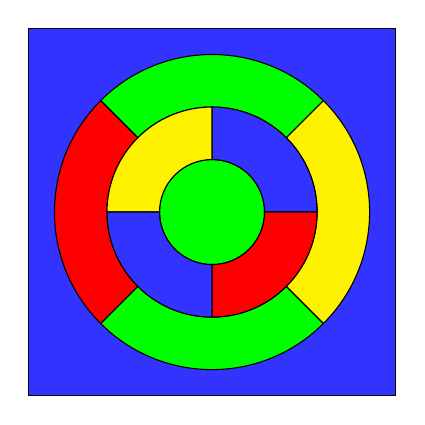
\begin{tikzpicture}[scale=.667]
\draw[fill=blue!80] (-3.5,-3.5) rectangle +(7,7);

\draw[fill=green] (0:1) 
  arc [start angle=0,  end angle=360, radius=1];

\draw[fill=green] (45:2) --
      (45:3)  arc[start angle=45,  end angle=135, radius=3] --
      (135:2) arc[start angle=135, end angle=45,  radius=2];
\draw[fill=green] (-45:2) --
      (-45:3)  arc[start angle=-45,  end angle=-135, radius=3] --
      (-135:2) arc[start angle=-135, end angle=-45,  radius=2];
\draw[fill=yellow] (45:2) --
      (45:3)  arc[start angle=45,  end angle=-45, radius=3] --
      (-45:2) arc[start angle=-45, end angle=45,  radius=2];
\draw[fill=red] (135:2) --
      (135:3)  arc[start angle=135,  end angle=225, radius=3] --
      (225:2) arc[start angle=225, end angle=135,  radius=2];

\draw[fill=blue!80] (0:1) --
      (0:2)  arc[start angle=0,  end angle=90, radius=2] --
      (90:1) arc[start angle=90, end angle=0,  radius=1];
\draw[fill=red] (0:1) --
      (0:2)  arc[start angle=0,  end angle=-90, radius=2] --
      (-90:1) arc[start angle=-90, end angle=0,  radius=1];
\draw[fill=yellow] (90:1) --
      (90:2)  arc[start angle=90,  end angle=180, radius=2] --
      (180:1) arc[start angle=180, end angle=90,  radius=1];
\draw[fill=blue!80] (180:1) --
      (180:2)  arc[start angle=180,  end angle=270, radius=2] --
      (270:1) arc[start angle=270, end angle=180,  radius=1];
\end{tikzpicture}
%\includegraphics[width=0.8\textwidth]{Fig4_1b}
         \captionof{figure}{Coloriage d'une carte planaire avec quatre  couleurs.}\label{f.five-planar-map-four}
     \end{minipage}

\vspace{0.4cm}



\begin{definition}
Un \emph{graphe} est un ensemble de sommets $S$ et un ensemble d'arêtes $A$, tels que chaque arête ait exactement deux sommets.

Un \emph{graphe planaire} est un graphe tel qu'aucune arête ne se croise. Dans un graphe planaire, les zones délimitées par un ensemble d'arêtes sont appelées \emph{faces}.

Un \emph{coloriage} d'un graphe planaire est une attribution de couleurs aux sommets telle que deux sommets de même couleur ne soient pas reliés par une arête.
\end{definition}

Les cartes planaires et les graphes planaires sont duaux et il est pratique d'étudier les problèmes de coloriage dans les graphes plutôt que dans les cartes.

\begin{theorem}
Étant donné une carte planaire, on peut construire un graphe planaire tel que pour chaque coloriage des régions de la carte, il existe un coloriage des sommets du graphe, et inversement.
\end{theorem}

\begin{proof}
Construire un sommet pour chaque région et construire une arête entre deux sommets si et seulement si les régions correspondantes partagent une frontière. 
\end{proof}

\begin{example}
La figure~\ref{f.five-planar-graph-map} montre la carte planaire de la figure~\ref{f.five-planar-map-four} et les sommets associés aux régions. La figure~\ref{f.five-planar-graph-graph} montre le graphe planaire qui correspond à la carte.
\end{example}

\vspace{0.4cm}

\begin{minipage}{0.4\textwidth}
\centering    
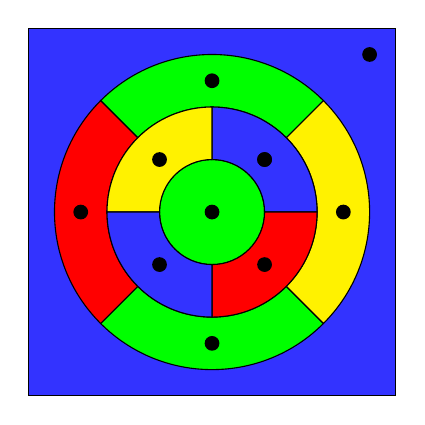
\begin{tikzpicture}[scale=.667]

\draw[fill=blue!80] (-3.5,-3.5) rectangle +(7,7);

\draw[fill=green] (0:1) 
  arc [start angle=0,  end angle=360, radius=1];

\draw[fill=green] (45:2) --
      (45:3)  arc[start angle=45,  end angle=135, radius=3] --
      (135:2) arc[start angle=135, end angle=45,  radius=2];
\draw[fill=green] (-45:2) --
      (-45:3)  arc[start angle=-45,  end angle=-135, radius=3] --
      (-135:2) arc[start angle=-135, end angle=-45,  radius=2];
\draw[fill=yellow] (45:2) --
      (45:3)  arc[start angle=45,  end angle=-45, radius=3] --
      (-45:2) arc[start angle=-45, end angle=45,  radius=2];
\draw[fill=red] (135:2) --
      (135:3)  arc[start angle=135,  end angle=225, radius=3] --
      (225:2) arc[start angle=225, end angle=135,  radius=2];

\draw[fill=blue!80] (0:1) --
      (0:2)  arc[start angle=0,  end angle=90, radius=2] --
      (90:1) arc[start angle=90, end angle=0,  radius=1];
\draw[fill=red] (0:1) --
      (0:2)  arc[start angle=0,  end angle=-90, radius=2] --
      (-90:1) arc[start angle=-90, end angle=0,  radius=1];
\draw[fill=yellow] (90:1) --
      (90:2)  arc[start angle=90,  end angle=180, radius=2] --
      (180:1) arc[start angle=180, end angle=90,  radius=1];
\draw[fill=blue!80] (180:1) --
      (180:2)  arc[start angle=180,  end angle=270, radius=2] --
      (270:1) arc[start angle=270, end angle=180,  radius=1];


\foreach \x/\y/\name in {
    0/0/O,
    3/3/Z,
    1/1/E,-1/1/F,-1/-1/G,1/-1/H,
    0/2.5/A,2.5/0/B,0/-2.5/C,-2.5/0/D,
    } {
  \fill (\x,\y) coordinate(\name) circle(4pt);
}
\end{tikzpicture}
%\includegraphics[width=0.8\textwidth]{Fig4_2a}
         \captionof{figure}{Association des sommets aux régions d'une carte planaire.}\label{f.five-planar-graph-map}
     \end{minipage}
     \hspace{3em}
     \begin{minipage}{0.4\textwidth}
\centering     
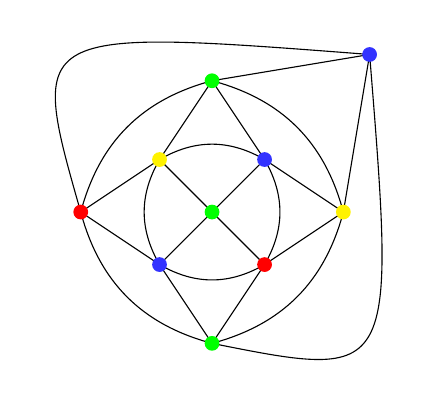
\begin{tikzpicture}[scale=.667]

\foreach \x/\y/\name in {
    0/0/O,
    3/3/Z,
    1/1/E,-1/1/F,-1/-1/G,1/-1/H,
    0/2.5/A,2.5/0/B,0/-2.5/C,-2.5/0/D,
    } {
  \coordinate(\name) at (\x,\y);
}

\draw (E) -- (O) -- (F);
\draw (G) -- (O) -- (H);
\draw (E) to [bend right=30] (F) to [bend right=30] (G) 
          to [bend right=30] (H) to [bend right=30] (E);
\draw (A) -- (E) -- (B) -- (H) -- (C) -- (G) -- (D) -- (F);
\draw (A) to [bend right=30] (D) to [bend right=30] (C) 
          to [bend right=30] (B) to [bend right=30] (A);

\draw (F) -- (A) -- (Z) -- (B);
\draw (C) .. controls (3.5,-3.2) .. (Z);
\draw (D) .. controls (-3.5,3.5) .. (Z);

\foreach \cl/\x/\y in {
    green/0cm/0cm,
    blue!80/3cm/3cm,
    blue!80/1cm/1cm,
    yellow/-1cm/1cm,
    blue!80/-1cm/-1cm,
    red/1cm/-1cm,
    green/0cm/2.5cm,
    yellow/2.5cm/0cm,
    green/0cm/-2.5cm,
    red/-2.5cm/0cm
    }
 \fill[\cl] (\x,\y) circle (4pt);
\end{tikzpicture}
%\includegraphics[width=0.8\textwidth]{Fig4_2b}
         \captionof{figure}{Le graphe planaire qui correspond à la carte planaire.}\label{f.five-planar-graph-graph}
     \end{minipage}

\vspace{0.4cm}



Nous pouvons encore limiter nos graphes à ceux dont les faces sont triangulaires.

\begin{definition}
Un graphe est \emph{triangulaire} si toutes ses faces sont délimitées par trois arêtes. Un graphe peut être \emph{triangulé} si des arêtes peuvent être ajoutées de sorte que le graphe soit triangulaire. On dit aussi qu'il existe une triangulation du graphe.
\end{definition}

\begin{example}
Les faces du graphe planaire de la figure~\ref{f.five-planar-graph-graph} sont triangulaires car chacune d'elles est délimitée par trois arêtes. Les arêtes sont courbées et les faces ne sont donc pas des triangles, qui sont des polygones dont les trois arêtes sont des segments de  droite.
\end{example}

\begin{advanced}
Le {\bf théorème de F\'{a}ry} stipule que tout graphe planaire triangulaire peut être transformé en un graphe planaire équivalent dont les arêtes sont des segments de droite. Par conséquent, sans perte de généralité, les démonstrations peuvent être limitées aux graphes planaires dont les faces sont des triangles.
\end{advanced}

\begin{example}
La figure~\ref{f.five-triangular-graph} (à gauche) montre qu'un carré peut être colorié avec deux couleurs, mais s'il est triangulé (au centre), quatre couleurs sont nécessaires. Notre objectif est de démontrer que tous les graphes peuvent être coloriés avec $n$ couleurs pour un certain $n$. Si le graphe triangulé est colorié avec $n$ couleurs, le graphe original l'est aussi, car la suppression des arêtes supplémentaires n'invalide pas le coloriage (à droite).
\end{example}

\begin{figure}[htbp]
\centering
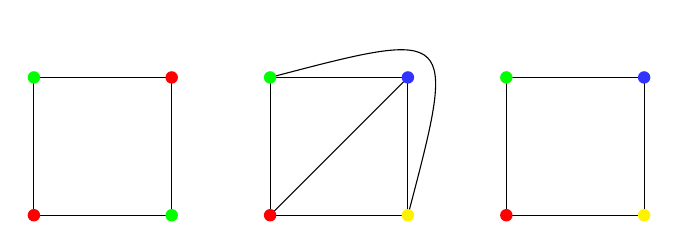
\begin{tikzpicture}[scale=.25]
\draw (-3.5,-3.5) rectangle +(7,7);
\fill[red] (-3.5,-3.5) circle(9pt);
\fill[green] (-3.5,3.5) circle(9pt);
\fill[green] (3.5,-3.5) circle(9pt);
\fill[red] (3.5,3.5) circle(9pt);
\begin{scope}[xshift=12cm]
\draw (-3.5,-3.5) -- (3.5,3.5);
\draw (-3.5,3.5) .. controls (6,6) .. (3.5,-3.5);
\draw (-3.5,-3.5) rectangle +(7,7);
\fill[red] (-3.5,-3.5) circle(9pt);
\fill[green] (-3.5,3.5) circle(9pt);
\fill[yellow] (3.5,-3.5) circle(9pt);
\fill[blue!80] (3.5,3.5) circle(9pt);
\end{scope}
\begin{scope}[xshift=24cm]
\draw (-3.5,-3.5) rectangle +(7,7);
\fill[red] (-3.5,-3.5) circle(9pt);
\fill[green] (-3.5,3.5) circle(9pt);
\fill[yellow] (3.5,-3.5) circle(9pt);
\fill[blue!80] (3.5,3.5) circle(9pt);
\end{scope}
\end{tikzpicture}
%\includegraphics[width=\textwidth]{Fig4_3}
\caption{Coloriage d'un graphe triangulé.}
\label{f.five-triangular-graph}
\end{figure}

\section{La formule d'Euler}\label{s.euler}

\begin{theorem}\label{thm.euler} Soit $G$ un graphe planaire connexe avec $S$ sommets, $A$ arêtes et $F$ faces. Alors $S-A+F=2$.
\end{theorem}

\begin{proof}
Par récurrence sur le nombre d'arêtes. Si le nombre d'arêtes du graphe est nul, il n'y a qu'un seul sommet et une seule face, donc $1-0+1=2$. Sinon, il y a au moins une arête $a$ et elle relie deux sommets $s_1$ et $s_2$. Supprimons  l'arête $a$.

\textit{Premier cas:}
Le graphe devient non connexe (fig.~\ref{f.five-disconnected-removing}). Fusionnons $s_1$ avec $s_2$ (fig.~\ref{f.five-disconnected-merge}). Le graphe résultant $G'$ est un graphe planaire connexe qui  possède moins d'arêtes que $G$, donc par hypothèse de récurrence $(S-1)-(A-1)+F=2$ puisque le nombre de sommets est également réduit de un. En simplifiant, on obtient $S-A+F=2$ pour $G$.

\vspace{0.3cm}

\begin{minipage}{0.4\textwidth}
\centering   
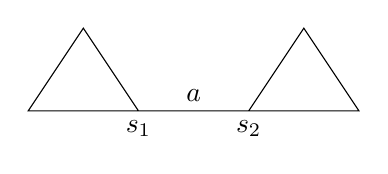
\begin{tikzpicture}[scale=.7]
\draw (2,0) -- (1,1.5) -- (0,0) -- (2,0) node[below] {$s_1$} -- node[above] {$a$} (4,0) node[below] {$s_2$} -- (6,0) -- (5,1.5) -- (4,0);
\end{tikzpicture}
%\includegraphics[width=\textwidth]{Fig4_4a}
         \captionof{figure}{La suppression d'une arête rend le graphe non connexe.}\label{f.five-disconnected-removing}   
     \end{minipage}
     \hspace{3em}
     \begin{minipage}{0.4\textwidth}
\centering         
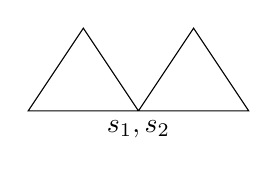
\begin{tikzpicture}[scale=.7]
\draw (2,0) -- (1,1.5) -- (0,0) -- (2,0) node[below] {$s_1,s_2$} -- (4,0) -- (3,1.5) -- (2,0);
\end{tikzpicture}
%\includegraphics[width=\textwidth]{Fig4_4b}
         \captionof{figure}{Fusion de deux sommets.}\label{f.five-disconnected-merge}
     \end{minipage}
     
\vspace{0.4cm}



\textit{Deuxième cas:}
Le graphe reste connexe (fig.~\ref{f.five-connected-remains}). $G'$ a moins d'arêtes que $G$ (fig.~\ref{f.five-connected-fewer}), donc par hypothèse de récurrence $S-(A-1)+(F-1)=2$ puisque enlever l'arête joint deux faces en une. En simplifiant, on obtient $S-A+F=2$ pour $G$.
\end{proof}

\vspace{0.4cm}

\begin{minipage}{0.4\textwidth}
\centering     
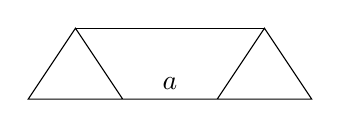
\begin{tikzpicture}[scale=.6]
\draw (2,0) -- (1,1.5) -- (0,0) -- (2,0) -- node[above] {$a$} (4,0) -- (6,0) -- (5,1.5) -- (4,0);
\draw (1,1.5) -- (5,1.5);
\end{tikzpicture}
%\includegraphics[width=\textwidth]{Fig4_5a}
         \captionof{figure}{La suppression d'une arête ne rend pas le graphe non connexe.}\label{f.five-connected-remains}
         
     \end{minipage}
     \hspace{3em}
     \begin{minipage}{0.4\textwidth}
\centering    
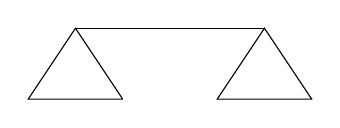
\begin{tikzpicture}[scale=.6]
\draw (2,0) -- (1,1.5) -- (0,0) -- (2,0);
\draw (4,0) -- (5,1.5) -- (6,0) -- cycle;
\draw (1,1.5) -- (5,1.5);
\end{tikzpicture}
%\includegraphics[width=\textwidth]{Fig4_5b}
         \captionof{figure}{Le graphe reste connexe et comporte moins d'arêtes.}\label{f.five-connected-fewer}
     \end{minipage}

\vspace{0.4cm}





\begin{theorem}\label{th43}
Soit $G$ un graphe planaire connexe et triangulé avec $A$ arêtes et $S$ sommets. Alors $A= 3S-6$.
\end{theorem}
\begin{proof}
Chaque face est délimitée par trois arêtes, donc $A=3F/2$, où nous avons divisé par $2$ car chaque arête a été comptée deux fois, une fois pour chaque face qu'elle délimite. D'après la formule d'Euler,
\begin{align*}
A&=S+F-2\\
&=S+2A/3-2,\\
A&=3S-6\,.\qedhere
\end{align*}
\end{proof}

\begin{example}
Le graphe planaire de la figure~\ref{f.five-planar-graph-graph} possède $10$ sommets et $3\cdot 10-6=24$ arêtes.
\end{example}

\begin{theorem}\label{thm.count}
Soit $G$ un graphe planaire connexe. Alors $A\leq 3S-6$.
\end{theorem}

\begin{proof}
Triangulons $G$ pour obtenir $G'$. D'après le théorème~\ref{th43}, $A'= 3S'-6$. Supprimons maintenant des arêtes de $G'$ pour obtenir $G$. Le nombre de sommets ne change pas, donc $A\leq 3S-6$.
\end{proof}

\begin{example}
Le graphe de la figure~\ref{f.five-fewer} a 8 arêtes et 6  sommets et $8< 3\cdot 6 - 6= 12$.
La figure~\ref{f.five-upper-limit} montre un graphe triangulé avec $6$ sommets et $3\cdot 6 - 6= 12$ arêtes.
\end{example}

\vspace{0.4cm}

\begin{minipage}{0.4\textwidth}
\centering  
\begin{tikzpicture}[scale=.6]
\draw (2,0) -- (1,1.5) -- (0,0) -- (2,0) -- (4,0) -- (6,0) -- (5,1.5) -- (4,0);
\draw (1,1.5) -- (5,1.5);
\path (2,0) .. controls (-1,-1) and (-1,1) .. (1,1.5);
\path (2,0) .. controls (3,-1) .. (6,0) .. controls (7,2) and (4,2) .. (1,1.5);
\end{tikzpicture}
%\includegraphics[width=\textwidth]{Fig4_6a}
         \captionof{figure}{Moins d'arêtes que la borne supérieure}
         \label{f.five-fewer}       
     \end{minipage}
     \hspace{3em}
     \begin{minipage}{0.4\textwidth}
\centering   
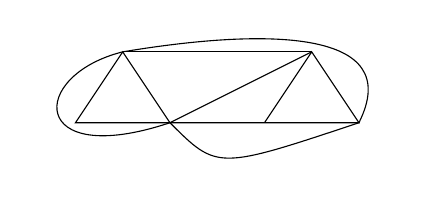
\begin{tikzpicture}[scale=.6]
\draw (2,0) -- (1,1.5) -- (0,0) -- (2,0) -- (4,0) -- (6,0) -- (5,1.5) -- (4,0);
\draw (1,1.5) -- (5,1.5);
\draw (2,0) -- (5,1.5);
\draw (2,0) .. controls (-1,-1) and (-1,1) .. (1,1.5);
\draw (2,0) .. controls (3,-1) .. (6,0) .. controls (7,2) and (4,2) .. (1,1.5);
\end{tikzpicture}
%\includegraphics[width=\textwidth]{Fig4_6b}
         \captionof{figure}{Dans un graphe triangulé, le nombre d'arêtes est maximal.}
         \label{f.five-upper-limit}
     \end{minipage}

\vspace{0.4cm}


\section{Graphes non planaires}\label{s.nonplanar}

Faisons un petit détour pour montrer comment les théorèmes~\ref{thm.euler} et~\ref{thm.count} peuvent être utilisés pour démontrer que certains graphes ne sont pas planaires.

\begin{theorem}
$K_5$, le graphe complet à cinq sommets, n'est pas planaire (fig.~\ref{f.five-k5}).
\end{theorem}

\vspace{0.4cm}

\begin{minipage}{0.4\textwidth}
\centering      
\begin{tikzpicture}[scale=.8]
\node (pentagon) [minimum size=4cm,regular polygon,regular polygon sides=5] at (0,0) {};
\draw (pentagon.corner 1) -- (pentagon.corner 2);
\draw (pentagon.corner 2) -- (pentagon.corner 3);
\draw (pentagon.corner 3) -- (pentagon.corner 4);
\draw (pentagon.corner 4) -- (pentagon.corner 5);
\draw (pentagon.corner 5) -- (pentagon.corner 1);
\draw (pentagon.corner 1) -- (pentagon.corner 3);
\draw (pentagon.corner 1) -- (pentagon.corner 4);
\draw (pentagon.corner 2) -- (pentagon.corner 4);
\draw (pentagon.corner 2) -- (pentagon.corner 5);
\draw (pentagon.corner 3) -- (pentagon.corner 5);
\end{tikzpicture}
%\includegraphics[width=0.8\textwidth]{Fig4_7a}
         \captionof{figure}{$K_5$ n'est pas planaire.}\label{f.five-k5}
     \end{minipage}
     \hspace{3em}
     \begin{minipage}{0.4\textwidth}
\centering       
\begin{tikzpicture}[scale=.6]
\node (pentagon) [minimum size=4cm,regular polygon,regular polygon sides=5] at (0,0) {};
\draw (pentagon.corner 1) -- (pentagon.corner 2);
\draw (pentagon.corner 2) -- (pentagon.corner 3);
\draw (pentagon.corner 3) -- (pentagon.corner 4);
\draw (pentagon.corner 4) -- (pentagon.corner 5);
\draw (pentagon.corner 5) -- (pentagon.corner 1);
\draw (pentagon.corner 1) .. controls (-4,1) .. 
      (pentagon.corner 3);
\draw (pentagon.corner 1) .. controls (4,1) ..
      (pentagon.corner 4);
\draw (pentagon.corner 2) -- (pentagon.corner 4);
\draw (pentagon.corner 2) -- (pentagon.corner 5);
\draw (pentagon.corner 3) -- (pentagon.corner 5);
\draw[thick] (0,-.95) circle(5pt);
\end{tikzpicture}
%\includegraphics[width=0.8\textwidth]{Fig4_7b}
         \captionof{figure}{Une tentative ratée de dessiner $K_5$ comme un graphe  planaire.}\label{f.five-k5-failed}
     \end{minipage}

\vspace{0.4cm}



\begin{proof}
Pour $K_5$, $S=5$ et $A=10$. D'après le théorème~\ref{thm.count}, le nombre d'arêtes devrait être inférieur ou égal à $3\cdot 5 -6=9$. Donc le graphe n'est pas planaire.
\end{proof}

\begin{theorem}
$K_{3,3}$, le graphe bipartite avec trois sommets de chaque côté, n'est pas planaire (fig.~\ref{f.five-k33}).
\end{theorem}

\vspace{0.4cm}

\begin{minipage}{0.4\textwidth}
\centering      
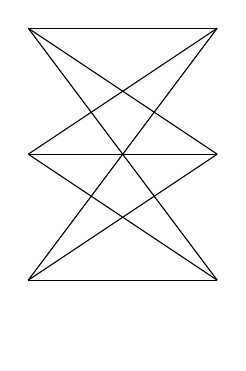
\begin{tikzpicture}[scale=.8]
\draw (0,0) -- (3,0);
\draw (0,2) -- (3,2);
\draw (0,4) -- (3,4);
\draw (0,0) -- (3,2);
\draw (0,2) -- (3,4);
\draw (0,4) -- (3,0);
\draw (0,0) -- (3,4);
\draw (0,2) -- (3,0);
\draw (0,4) -- (3,2);
\path (0,-1) -- (3,-1);
\end{tikzpicture}
%\includegraphics[width=0.6\textwidth]{Fig4_8a}
         \captionof{figure}{$K_{3,3}$ n'est pas planaire.}
         \label{f.five-k33}         
     \end{minipage}
     \hspace{3em}
     \begin{minipage}{0.4\textwidth}
\centering     
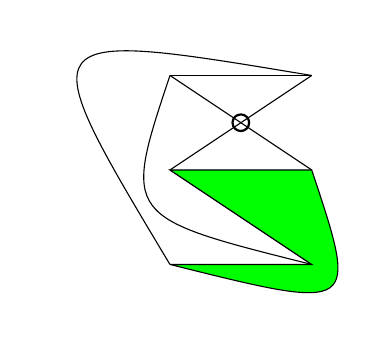
\begin{tikzpicture}[scale=.6]
\draw (0,4) -- (3,4);
\draw (0,2) -- (3,4);
\draw (0,4) .. controls (-1,1) .. (3,0);
\draw (0,0) .. controls (-3,5) .. (3,4);
\draw (0,2) -- (3,0);
\draw (0,4) -- (3,2);

\draw[fill=green] (0,0) -- (3,0) -- (3,0) -- (0,2)  -- (3,2) .. controls (4,-1) .. (0,0);
\draw[thick] (1.5,3) circle(5pt);
\end{tikzpicture}
%\includegraphics[width=0.8\textwidth]{Fig4_8b}
         \captionof{figure}{Une tentative ratée de dessiner $K_{3,3}$ comme un graphe planaire.}\label{f.five-k33-failed}
     \end{minipage}

\vspace{0.4cm}



\begin{proof}
$S=6$ et $A=9$. D'après le théorème~\ref{thm.euler}, si $K_{3,3}$ était  planaire, on aurait $F=A-S+2=9-6+2=5$. Mais chaque face est délimitée par quatre arêtes (fig.~\ref{f.five-k33-failed}), donc $A=4F/2=10\neq 9$.
\end{proof}

En 1930, Kazimierz Kuratowski a démontré la réciproque de ces théorèmes : si un graphe n'est pas planaire, il contient (dans un certain sens) $K_5$ ou $K_{3,3}$.

\section{Les degrés des sommets}\label{s.degrees}

\begin{definition}
$d(s)$, le \emph{degré} du sommet $s$, est le nombre d'arêtes incidentes en $s$.
\end{definition}

\begin{example}
Le graphe de la figure~\ref{f.five-planar-graph-graph} contient $8$ sommets correspondant aux deux anneaux et chaque sommet est de degré $5$. Le sommet correspondant à la face extérieure est de degré $4$ tout comme le sommet correspondant à la face intérieure. Par conséquent :
\[
\sum_{s\in S} d(s) = 5\cdot 8 + 4\cdot 2=48\,.
\]
Pour obtenir le nombre total d'arêtes, divisons 48 par $2$ car chaque arête a été comptée deux fois, une fois pour chacun des sommets auxquels elle est reliée.
\end{example}



En généralisant l'argument, on obtient :
\begin{theorem}\label{thm.degrees}
Soit $d_i$ pour $i\in \{1,2,3,\ldots,k\}$ le nombre de sommets de degré $i$ dans un graphe planaire connexe $G$ avec $S$ sommets et $A$ arêtes, où $k$ est le  degré maximal d'un sommet dans $S$. Alors 
\[
\sum_{s\in S} d(s) =\sum_{i=1}^{k} i\cdot d_i=2A\,.
\]
\end{theorem}

\begin{theorem}\label{thm.degree5}
Soit $G$ un graphe planaire connexe avec $A$ arêtes et $S$ sommets, et soit $d_i$ pour $i$ dans $\{1,2,3,\ldots,k\}$ le nombre de sommets de degré $i$, où $k$ est le plus haut degré d'un sommet dans $S$. Alors il existe un sommet $s$ dans $S$ tel que $d(s) \leq 5$.
\end{theorem}

\noindent \emph{Démonstration (première méthode)}. 
S'il existe $d_1$ sommets de degré $1$, $d_2$ sommets de degré $2$, \ldots, $d_k$ sommets de degré $k$, alors $S=\sum_{i=1}^{k}d_i$.  D'après les théorèmes~\ref{thm.count} et \ref{thm.degrees},
\[
\sum_{i=1}^{k} i\cdot d_i=2A\leq 2(3S-6) = 6S-12=6\sum_{i=1}^{k} d_i -12\,.
\]
Par conséquent,
%
\begin{align*}
\sum_{i=1}^{k} i\cdot d_i &\leq 6\sum_{i=1}^{k} d_i -12\\
\sum_{i=1}^{k} (6-i)d_i&\geq 12\,.
\end{align*}
Puisque $12>0$ et puisque tous les $d_i$ sont positifs ou nuls, pour au moins un $i$ on a $6-i>0$ et donc $i<6$.\qed

\medskip 

\noindent  \emph{Démonstration (deuxième méthode)}. 
Calculons le degré moyen des sommets qui est la somme des degrés divisée par le nombre de sommets :
\[
d_{\textit{\footnotesize moy}}=\frac{\sum_{i=1}^{k} i\cdot d_i}{S}\,.
\]
Mais la somme des degrés est le double du nombre d'arêtes, ce qui donne d'après le  théorème~\ref{thm.count} :
\[
d_{\textit{\footnotesize moy}}=\frac{2A}{S}\leq \frac{6S-12}{S}=6-\frac{6}{S}<6\,.
\]
Si la moyenne est strictement inférieure à six, il doit y avoir un sommet de degré strictement  inférieur à six.\qed

\begin{example}
Dans la figure~\ref{f.five-planar-graph-graph}, la somme des degrés est de $8\cdot 5 + 2\cdot 4=48$. Comme il y a $10$ sommets, le degré moyen est de $48/10=\mbox{4,8}$ et il doit y avoir un sommet de degré 4 ou moins.
\end{example}

\section{Le théorème des six couleurs}\label{s.six-color}

\begin{theorem}\label{thm.sixcolor}
Tout graphe planaire $G$ peut être colorié avec six couleurs.
\end{theorem}
\begin{proof}
Par récurrence sur le nombre de sommets. Si $G$ a six sommets ou moins, six couleurs suffisent.
Pour l'étape de récurrence, d'après le théorème~\ref{thm.degree5}, $G$ a un sommet $s$ avec un degré inférieur ou égal à $5$. Supprimons le sommet $s$ pour obtenir le graphe $G'$. Par hypothèse de récurrence, $G'$ peut être colorié avec six couleurs, mais $s$ a au plus $5$ voisins et au plus $5$ couleurs sont utilisées pour les colorier (fig.~\ref{f.five-six-five}), donc $s$ peut être colorié en utilisant la sixième couleur (fig.~\ref{f.five-six-six}).
\end{proof}

\vspace{0.2cm}

\begin{minipage}{0.4\textwidth}
\centering   
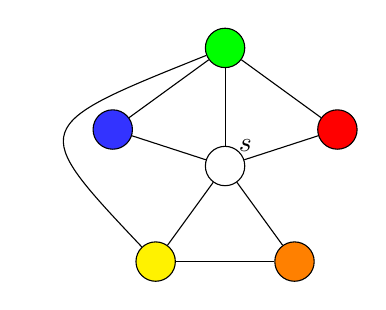
\begin{tikzpicture}[scale=.5,minimum size=5mm,inner sep=0pt]
\foreach \name/\color/\theta in
    {A/red/18,B/green/90,C/blue!80/162,D/yellow/234,E/orange/306}
  \node[circle,draw,fill=\color] (\name) at (\theta:3) {};
\node[circle,draw] (O) at (0,0) {};
\node[above right] at (O) {$s$};
\foreach \name in {A,B,C,D,E}
  \draw (O) -- (\name);
\foreach \i/\j in {A/B,B/C,D/E}
  \draw (\i) -- (\j);
\draw (B) .. controls (-5,1) .. (D);
\end{tikzpicture}
%\includegraphics[width=\textwidth]{Fig4_9a}
         \captionof{figure}{Cinq couleurs suffisent pour colorier les voisins de $s$.}\label{f.five-six-five}
         
     \end{minipage}
     \hspace{3em}
     \begin{minipage}{0.4\textwidth}
\centering     
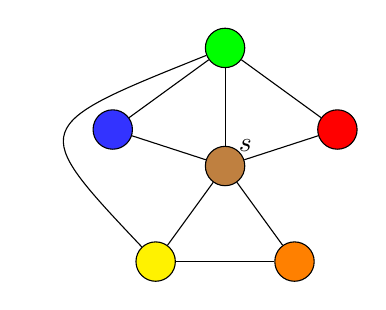
\begin{tikzpicture}[scale=.5,minimum size=5mm,inner sep=0pt]
\foreach \name/\color/\theta in
    {A/red/18,B/green/90,C/blue!80/162,D/yellow/234,E/orange/306}
  \node[circle,draw,fill=\color] (\name) at (\theta:3) {};
\node[circle,draw,fill=brown] (O) at (0,0) {};
\node[above right] at (O) {$s$};
\foreach \name in {A,B,C,D,E}
  \draw (O) -- (\name);
\foreach \i/\j in {A/B,B/C,D/E}
  \draw (\i) -- (\j);
\draw (B) .. controls (-5,1) .. (D);
\end{tikzpicture}
%\includegraphics[width=\textwidth]{Fig4_9b}
         \captionof{figure}{Coloriage de $s$ avec la sixième couleur.}\label{f.five-six-six}
     \end{minipage}




\section{Le théorème des cinq couleurs}\label{s.five-color}

\begin{definition}
Soit $G$ un graphe planaire coloré. Une \emph{chaîne} (de Kempe) $G'$ est un sous-graphe maximal, colorié avec deux couleurs et connexe de $G$.
\end{definition}

 
\begin{theorem}\label{thm.fivecolor}
Tout graphe planaire $G$ peut être colorié avec cinq couleurs.
\end{theorem}

\begin{proof}
Par récurrence sur le nombre de sommets. Si $G$ a cinq sommets ou moins, cinq couleurs suffisent.
Pour l'étape de récurrence, d'après le théorème~\ref{thm.degree5}, $G$ a un sommet $s$ avec un degré inférieur ou égal à $5$. Supprimons $s$ pour obtenir $G'$. Par l'hypothèse de récurrence, $G'$ peut être colorié avec cinq couleurs. Dans $G$, si le degré de $s$ est strictement inférieur à $5$, ou si $s_1,\ldots,s_5$, les voisins de $s$, sont coloriés avec quatre couleurs ou moins, $s$ peut être colorié avec la cinquième couleur.
Sinon, $s_1,\ldots,s_5$ sont coloriés avec des couleurs différentes dans $G'$ (fig.~\ref{f.five-color-proof}, en haut).

\begin{figure}[htbp]
\centering     
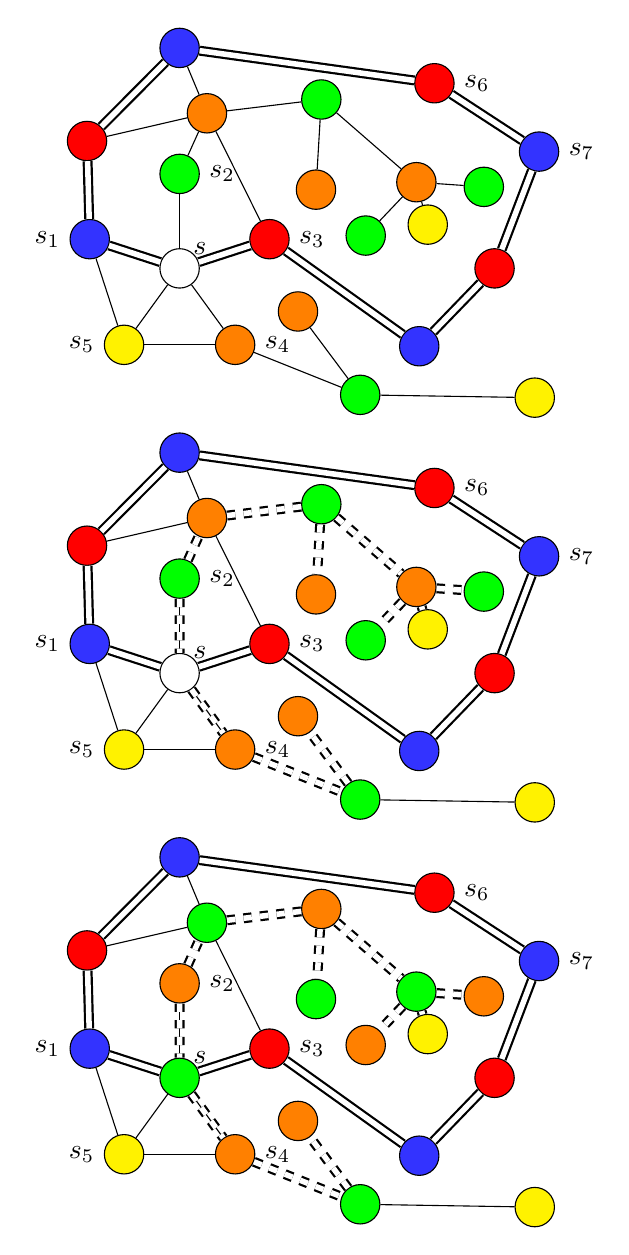
\begin{tikzpicture}[scale=.4,minimum size=5mm,inner sep=0pt]
\foreach \name/\color/\theta in
    {A/red/18,B/green/90,C/blue!80/162,D/yellow/234,E/orange/306}
  \node[circle,draw,fill=\color] (\name) at (\theta:3) {};
\node[circle,draw] (O) at (0,0) {};
\node[above right] at (O) {$s$};

\node[right,xshift=8pt] at (A) {$s_3$};
\node[right,xshift=8pt] at (B) {$s_2$};
\node[left,,xshift=-8pt] at (C) {$s_1$};
\node[left,,xshift=-8pt] at (D) {$s_5$};
\node[right,xshift=8pt] at (E) {$s_4$};

\foreach \name in {A,B,C,D,E}
  \draw (O) -- (\name);
  
\node[circle,draw,fill=red]  (X1) at (126:5) {};
\node[circle,draw,fill=blue!80] (X2) at (90:7)  {};
\node[circle,draw,fill=red]  (X3) at (36:10) {};
\node[right,xshift=8pt] at (X3) {$s_6$};
\node[circle,draw,fill=blue!80] (X4) at (18:12) {};
\node[right,xshift=8pt] at (X4) {$s_7$};
\node[circle,draw,fill=red]  (X5) at (0:10) {};
\node[circle,draw,fill=blue!80] (X6) at (-18:8) {};
\draw[thick,double distance=2pt] (C)  -- (X1);
\draw[thick,double distance=2pt] (X1) -- (X2);
\draw[thick,double distance=2pt] (X2) -- (X3);
\draw[thick,double distance=2pt] (X3) -- (X4);
\draw[thick,double distance=2pt] (X4) -- (X5);
\draw[thick,double distance=2pt] (X5) -- (X6);
\draw[thick,double distance=2pt] (X6) -- (A);
\draw[thick,double distance=2pt] (A) -- (O) -- (C);

\node[circle,draw,fill=orange]  (Y1)  at (80:5) {};
\node[circle,draw,fill=green]   (Y2)  at (50:7)  {};
\node[circle,draw,fill=orange]  (Y3A) at (20:8) {};
\node[circle,draw,fill=orange]  (Y3B) at (30:5) {};
\node[circle,draw,fill=green]   (Y4A) at (10:6) {};
\node[circle,draw,fill=yellow]  (Y4B) at (10:8) {};
\node[circle,draw,fill=green]   (Y4C) at (15:10) {};
\node[circle,draw,fill=green]   (Y5)  at (-35:7) {};
\node[circle,draw,fill=yellow]  (Y6A) at (-20:12) {};
\node[circle,draw,fill=orange]  (Y6B) at (-20:4) {};
\draw (B)  -- (Y1);
\draw (Y1) -- (Y2);
\draw (Y2) -- (Y3A);
\draw (Y2) -- (Y3B);
\draw (Y3A) -- (Y4A);
\draw (Y3A) -- (Y4B);
\draw (Y3A) -- (Y4C);
\draw (E)  -- (Y5);
\draw (Y5) -- (Y6A);
\draw (Y5) -- (Y6B);
\draw (A) -- (Y1);
\draw (X2) -- (Y1);
\draw (X1) -- (Y1);
\draw (D) -- (E);
\draw (D) -- (C);

\begin{scope}[yshift=-12.85cm]
\foreach \name/\color/\theta in
    {A/red/18,B/green/90,C/blue!80/162,D/yellow/234,E/orange/306}
  \node[circle,draw,fill=\color] (\name) at (\theta:3) {};
\node[circle,draw] (O) at (0,0) {};
\node[above right] at (O) {$s$};

\node[right,xshift=8pt] at (A) {$s_3$};
\node[right,xshift=8pt] at (B) {$s_2$};
\node[left,,xshift=-8pt] at (C) {$s_1$};
\node[left,,xshift=-8pt] at (D) {$s_5$};
\node[right,xshift=8pt] at (E) {$s_4$};

\foreach \name in {A,B,C,D,E}
  \draw (O) -- (\name);
  
\node[circle,draw,fill=red]  (X1) at (126:5) {};
\node[circle,draw,fill=blue!80] (X2) at (90:7)  {};
\node[circle,draw,fill=red]  (X3) at (36:10) {};
\node[circle,draw,fill=blue!80] (X4) at (18:12) {};
\node[circle,draw,fill=red]  (X5) at (0:10) {};
\node[circle,draw,fill=blue!80] (X6) at (-18:8) {};

\draw[thick,double distance=2pt] (C)  -- (X1);
\draw[thick,double distance=2pt] (X1) -- (X2);
\draw[thick,double distance=2pt] (X2) -- (X3);
\draw[thick,double distance=2pt] (X3) -- (X4);
\draw[thick,double distance=2pt] (X4) -- (X5);
\draw[thick,double distance=2pt] (X5) -- (X6);
\draw[thick,double distance=2pt] (X6) -- (A);
\draw[thick,double distance=2pt] (A) -- (O) -- (C);

\node[circle,draw,fill=orange]  (Y1)  at (80:5) {};
\node[circle,draw,fill=green]   (Y2)  at (50:7)  {};
\node[circle,draw,fill=orange]  (Y3A) at (20:8) {};
\node[circle,draw,fill=orange]  (Y3B) at (30:5) {};
\node[circle,draw,fill=green]   (Y4A) at (10:6) {};
\node[circle,draw,fill=yellow]   (Y4B) at (10:8) {};
\node[circle,draw,fill=green]   (Y4C) at (15:10) {};
\node[circle,draw,fill=green]   (Y5)  at (-35:7) {};
\node[circle,draw,fill=yellow]  (Y6A) at (-20:12) {};
\node[circle,draw,fill=orange]  (Y6B) at (-20:4) {};
\draw[thick,dashed,double distance=2pt] (B)  -- (O) -- (E);
\draw[thick,dashed,double distance=2pt] (B)  -- (Y1);
\draw[thick,dashed,double distance=2pt] (Y1) -- (Y2);
\draw[thick,dashed,double distance=2pt] (Y2) -- (Y3A);
\draw[thick,dashed,double distance=2pt] (Y2) -- (Y3B);
\draw[thick,dashed,double distance=2pt] (Y3A) -- (Y4A);
\draw[thick,dashed,double distance=2pt] (Y3A) -- (Y4B);
\draw[thick,dashed,double distance=2pt] (Y3A) -- (Y4C);
\draw[thick,dashed,double distance=2pt] (E)  -- (Y5);
\draw[thick,dashed,double distance=2pt] (Y5) -- (Y6B);
\draw (Y5) -- (Y6A);
\draw (A) -- (Y1);
\draw (X2) -- (Y1);
\draw (X1) -- (Y1);
\draw (D) -- (E);
\draw (D) -- (C);
\node[right,xshift=8pt] at (X3) {$s_6$};
\node[right,xshift=8pt] at (X4) {$s_7$};
\end{scope}

\begin{scope}[yshift=-25.7cm]
\foreach \name/\color/\theta in
    {A/red/18,B/orange/90,C/blue!80/162,D/yellow/234,E/orange/306}
  \node[circle,draw,fill=\color] (\name) at (\theta:3) {};
\node[circle,draw,fill=green] (O) at (0,0) {};
\node[above right] at (O) {$s$};

\node[right,xshift=8pt] at (A) {$s_3$};
\node[right,xshift=8pt] at (B) {$s_2$};
\node[left,,xshift=-8pt] at (C) {$s_1$};
\node[left,,xshift=-8pt] at (D) {$s_5$};
\node[right,xshift=8pt] at (E) {$s_4$};

\foreach \name in {A,B,C,D,E}
  \draw (O) -- (\name);
  
\node[circle,draw,fill=red]  (X1) at (126:5) {};
\node[circle,draw,fill=blue!80] (X2) at (90:7)  {};
\node[circle,draw,fill=red]  (X3) at (36:10) {};
\node[circle,draw,fill=blue!80] (X4) at (18:12) {};
\node[circle,draw,fill=red]  (X5) at (0:10) {};
\node[circle,draw,fill=blue!80] (X6) at (-18:8) {};

\draw[thick,double distance=2pt] (C)  -- (X1);
\draw[thick,double distance=2pt] (X1) -- (X2);
\draw[thick,double distance=2pt] (X2) -- (X3);
\draw[thick,double distance=2pt] (X3) -- (X4);
\draw[thick,double distance=2pt] (X4) -- (X5);
\draw[thick,double distance=2pt] (X5) -- (X6);
\draw[thick,double distance=2pt] (X6) -- (A);
\draw[thick,double distance=2pt] (A) -- (O) -- (C);

\node[circle,draw,fill=green]  (Y1)  at (80:5) {};
\node[circle,draw,fill=orange]   (Y2)  at (50:7)  {};
\node[circle,draw,fill=green]  (Y3A) at (20:8) {};
\node[circle,draw,fill=green]  (Y3B) at (30:5) {};
\node[circle,draw,fill=orange]   (Y4A) at (10:6) {};
\node[circle,draw,fill=yellow]   (Y4B) at (10:8) {};
\node[circle,draw,fill=orange]   (Y4C) at (15:10) {};
\node[circle,draw,fill=green]   (Y5)  at (-35:7) {};
\node[circle,draw,fill=yellow]  (Y6A) at (-20:12) {};
\node[circle,draw,fill=orange]  (Y6B) at (-20:4) {};

\draw[thick,dashed,double distance=2pt] (B)  -- (O) -- (E);
\draw[thick,dashed,double distance=2pt] (B)  -- (Y1);
\draw[thick,dashed,double distance=2pt] (Y1) -- (Y2);
\draw[thick,dashed,double distance=2pt] (Y2) -- (Y3A);
\draw[thick,dashed,double distance=2pt] (Y2) -- (Y3B);
\draw[thick,dashed,double distance=2pt] (Y3A) -- (Y4A);
\draw[thick,dashed,double distance=2pt] (Y3A) -- (Y4B);
\draw[thick,dashed,double distance=2pt] (Y3A) -- (Y4C);
\draw[thick,dashed,double distance=2pt] (E)  -- (Y5);
\draw[thick,dashed,double distance=2pt] (Y5) -- (Y6B);


\draw (Y5) -- (Y6A);
\draw (A) -- (Y1);
\draw (X2) -- (Y1);
\draw (X1) -- (Y1);
\draw (D) -- (E);
\draw (D) -- (C);
\node[right,xshift=8pt] at (X3) {$s_6$};
\node[right,xshift=8pt] at (X4) {$s_7$};
\end{scope}
\end{tikzpicture}
%\includegraphics[width=0.66\textwidth]{Fig4_10a}\\
%\includegraphics[width=0.66\textwidth]{Fig4_10b}\\
%\includegraphics[width=0.66\textwidth]{Fig4_10c}
\caption{Démonstration du théorème des cinq couleurs.}
\label{f.five-color-proof}
\end{figure}



Considérons le sommet $s_1$ qui est colorié en bleu et le sommet $s_3$ qui est colorié en rouge. Si $s_1$ et $s_3$ ne sont pas reliés par un chemin bleu-rouge (disons si l'arête $\overline{s_6s_7}$ n'existait pas), nous pouvons échanger les couleurs le long du chemin de $s_1$ à $s_6$ et colorier $s$ en bleu. Sinon, on considère la chaîne bleu-rouge qui contient $s_1$ et $s_3$. En ajoutant $s$ et les arêtes $\overline{ss_1}$ et $\overline{ss_3}$, on obtient un chemin fermé $P$ (double ligne) qui divise le plan en une région \og intérieure\fg{} et une région \og extérieure\fg{}  (fig.~\ref{f.five-color-proof}, au milieu).

Considérons $s_2$ qui est colorié en vert et $s_4$ qui est colorié en orange. Ces sommets ne peuvent pas être contenus dans une seule chaîne verte-orange, car $s_2$ est à l'intérieur de $P$ et $s_4$ est à l'extérieur de $P$, donc tout chemin les reliant doit traverser $P$, ce qui contredit l'hypothèse selon laquelle le graphe est planaire. Par conséquent, ils doivent être contenus dans deux chaînes verte-orange non reliées (double ligne pointillée, dans la figure~\ref{f.five-color-proof}, au milieu).
Échangeons les couleurs sur la chaîne contenant $s_2$ et alors $s$ peut être colorié en vert pour obtenir un coloriage à cinq couleurs de $G$ (fig.~\ref{f.five-color-proof}, en bas).
\end{proof}

\begin{advanced}
L'affirmation selon laquelle un chemin continu allant de l'intérieur d'une courbe continue fermée $P$ à l'extérieur de $P$ doit couper $P$ est le 
 théorème de Jordan. Ce théorème est intuitivement évident mais difficile à démontrer.
\end{advanced}

\section[La démonstration erronée de Kempe du théorème des quatre couleurs]{La démonstration erronée de Kempe du théorème\\ des quatre couleurs}\label{s.kempe}

\begin{theorem}\label{thm.fourcolor}
Tout graphe planaire $G$ peut être colorié avec quatre couleurs.
\end{theorem}

\noindent \emph{Démonstration (fausse)}.  L'initialisation la récurrence et la majeure partie de la démonstration sont les mêmes que celles du théorème des cinq couleurs. Le nouveau cas à considérer est un sommet $s$ avec cinq voisins qui, par hypothèse de récurrence, peut être colorié avec quatre couleurs après avoir enlevé $s$.

Dans la figure~\ref{f.five-kempe1}, il y a deux sommets $s_2$ et $s_5$ coloriés en bleu. Considérons la chaîne bleu-vert contenant $s_2$ et la chaîne bleu-jaune contenant $s_5$. La chaîne bleu-vert est contenue dans le chemin fermé défini par la chaîne rouge-jaune contenant $s_1$ et $s_3$ (double ligne) et la chaîne bleu-jaune est contenue dans le chemin fermé défini par la chaîne rouge-vert contenant $s_1$ et $s_4$ (double ligne pointillée).

Échangeons les couleurs de la chaîne bleu-vert et de la chaîne bleu-jaune (fig.~\ref{f.five-kempe1-exchange}). Le résultat est que les voisins de $s$ sont coloriés avec les trois couleurs rouge, vert et jaune, laissant le bleu libre de colorier $s$. \qed

\vspace{0.4cm}

\begin{minipage}{0.4\textwidth}
\centering     
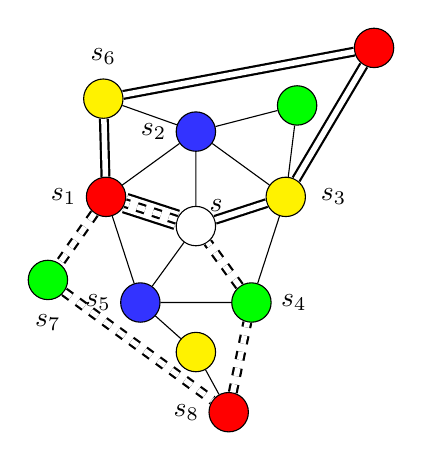
\begin{tikzpicture}[scale=.4,minimum size=5mm,inner sep=0pt]

% Draw center node and adjacent nodes
\foreach \name/\color/\theta in
    {A/yellow/18,B/blue!80/90,C/red/162,D/blue!80/234,E/green/306}
  \node[circle,draw,fill=\color] (\name) at (\theta:3) {};
\node[circle,draw] (O) at (0,0) {};
\node[above right]     at (O) {$s$};

\node[right,xshift=10pt] at (A) {$s_3$};
\node[left,xshift=-8pt]  at (B) {$s_2$};
\node[left,xshift=-8pt]  at (C) {$s_1$};
\node[left,xshift=-8pt]  at (D) {$s_5$};
\node[right,xshift=8pt]  at (E) {$s_4$};

% Draw red-yellow path
\node[circle,draw,fill=yellow]  (X1) at (126:5) {};
\node[circle,draw,fill=red] (X2) at (45:8)  {};

\draw[thick,double distance=2pt] 
  (C) -- (X1) -- (X2) -- (A) -- (O);
\draw[thick,double distance=6pt] (O) -- (C);

% Draw blue-green nodes within red-yellow path
\node[circle,draw,fill=green] (Y1)  at (50:5) {};

% Draw red-green path
\node[circle,draw,fill=green] (Z1)  at (-160:5) {};
\node[circle,draw,fill=red]   (Z2)  at (-80:6)  {};

\draw[thick,dashed,double distance=2pt] 
  (O) -- (C) -- (Z1) -- (Z2) -- (E) -- (O);

% Draw blue-yellow nodes within red-green path
\node[circle,draw,fill=yellow]   (U1)  at (-90:4)  {};

% Connect adjacent nodes not in paths
\draw (X1) -- (B) -- (Y1) -- (A) -- (B) -- 
      (C) -- (D) -- (E) -- (A);
\draw (Z2) -- (U1) -- (D) -- (O) -- (B);
\node[above,yshift=8pt] at (X1) {$s_6$};
\node[below,yshift=-8pt] at (Z1) {$s_7$};
\node[left,xshift=-8pt] at (Z2) {$s_8$};
\end{tikzpicture}
%\includegraphics[width=\textwidth]{Fig4_11a}
         \captionof{figure}{Chaînes de Kempe bleu-vert et bleu-jaune.}
         \label{f.five-kempe1}
     \end{minipage}
     \hspace{3em}
     \begin{minipage}{0.4\textwidth}
\centering    
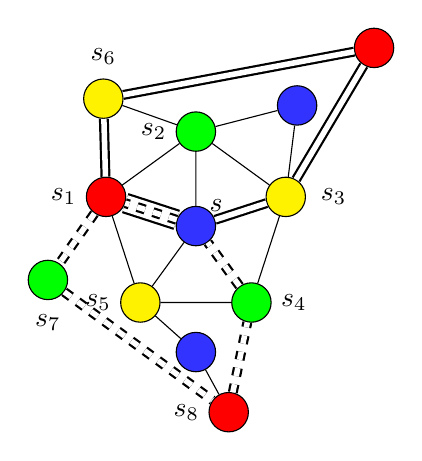
\begin{tikzpicture}[scale=.4,minimum size=5mm,inner sep=0pt]

% Draw center node and adjacent nodes
\foreach \name/\color/\theta in
    {A/yellow/18,B/green/90,C/red/162,D/yellow/234,E/green/306}
  \node[circle,draw,fill=\color] (\name) at (\theta:3) {};
\node[circle,draw,fill=blue!80] (O) at (0,0) {};
\node[above right]     at (O) {$s$};

\node[right,xshift=10pt] at (A) {$s_3$};
\node[left,xshift=-8pt]  at (B) {$s_2$};
\node[left,xshift=-8pt]  at (C) {$s_1$};
\node[left,xshift=-8pt]  at (D) {$s_5$};
\node[right,xshift=8pt]  at (E) {$s_4$};

% Draw red-yellow path
\node[circle,draw,fill=yellow]  (X1) at (126:5) {};
\node[circle,draw,fill=red] (X2) at (45:8)  {};

\draw[thick,double distance=2pt] 
  (C) -- (X1) -- (X2) -- (A) -- (O);
\draw[thick,double distance=6pt] (O) -- (C);

% Draw blue-green nodes within red-yellow path
\node[circle,draw,fill=blue!80] (Y1)  at (50:5) {};

% Draw red-green path
\node[circle,draw,fill=green] (Z1)  at (-160:5) {};
\node[circle,draw,fill=red]   (Z2)  at (-80:6)  {};

\draw[thick,dashed,double distance=2pt] 
  (O) -- (C) -- (Z1) -- (Z2) -- (E) -- (O);

% Draw blue-yellow nodes within red-green path
\node[circle,draw,fill=blue!80]   (U1)  at (-90:4)  {};

% Connect adjacent nodes not in paths
\draw (X1) -- (B) -- (Y1) -- (A) -- (B) -- 
      (C) -- (D) -- (E) -- (A);
\draw (Z2) -- (U1) -- (D) -- (O) -- (B);
\node[above,yshift=8pt] at (X1) {$s_6$};
\node[below,yshift=-8pt] at (Z1) {$s_7$};
\node[left,xshift=-8pt] at (Z2) {$s_8$};
\end{tikzpicture}
%\includegraphics[width=\textwidth]{Fig4_11b}
         \captionof{figure}{\'Echange des couleurs des deux chaînes de Kempe.}
         \label{f.five-kempe1-exchange}
     \end{minipage}

\vspace{0.4cm}



Heawood a remarqué que les chemins fermés définis par la chaîne rouge-jaune et la chaîne rouge-verte peuvent partager des sommets rouges ($s_1,s_8$ dans la figure~\ref{f.five-kempe2}). Lorsque les couleurs sont échangées dans les chaînes bleu-vert et bleu-jaune, il est possible que les sommets bleus $s_6$ et $s_7$ soient reliés (fig.~\ref{f.five-kempe2-share}) et le coloriage n'est plus correct.

\vspace{0.4cm}

\begin{minipage}{0.4\textwidth}
\centering     
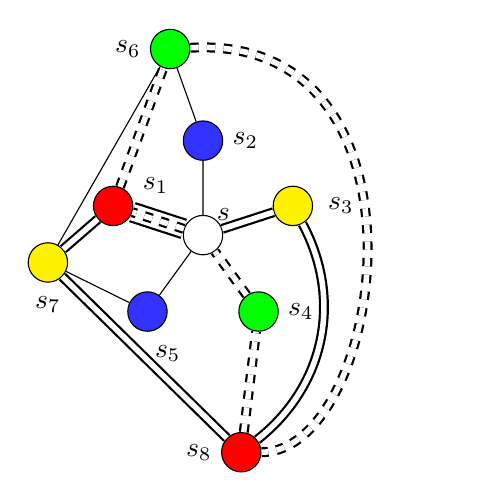
\begin{tikzpicture}[scale=.4,minimum size=5mm,inner sep=0pt]

% Draw center node and adjacent nodes
\foreach \name/\color/\theta in
    {A/yellow/18,B/blue!80/90,C/red/162,D/blue!80/234,E/green/306}
  \node[circle,draw,fill=\color] (\name) at (\theta:3) {};
\node[circle,draw] (O) at (0,0) {};
\node[above right]     at (O) {$s$};

\node[right,xshift=10pt] at (A) {$s_3$};
\node[right,xshift=8pt]  at (B) {$s_2$};
\node[above right,xshift=8pt]  at (C) {$s_1$};
\node[below right,yshift=-8pt] at (D) {$s_5$};
\node[right,xshift=8pt]  at (E) {$s_4$};

% Draw red-yellow path
\node[circle,draw,fill=yellow] (X1) at (-170:5) {};
\node[circle,draw,fill=red]    (X2) at (-80:7)  {};

\draw[thick,double distance=2pt] (A) -- (O);
\draw[thick,double distance=6pt] (O) -- (C);
\draw[thick,double distance=2pt] (C) --(X1) -- (X2);
\draw[thick,double distance=2pt,bend right=40] (X2) to (A);

% Draw red-green path
\node[circle,draw,fill=green] (Y1) at (100:6)  {};

\draw[dashed,thick,double distance=2pt] (O) -- (C) -- (Y1);
\draw[dashed,thick,double distance=2pt] 
  (Y1) .. controls (40:10) and (-50:9) .. (X2);
\draw[dashed,thick,double distance=2pt] (X2) -- (E) -- (O);

% Draw adjacent nodes
\draw (X1) -- (D) -- (O) -- (B) -- (Y1) -- (X1);
\node[left,xshift=-8pt] at (Y1) {$s_6$};
\node[below,yshift=-8pt] at (X1) {$s_7$};
\node[left,xshift=-8pt] at (X2) {$s_8$};
\end{tikzpicture}
%\includegraphics[width=\textwidth]{Fig4_12a}
         \captionof{figure}{Les chaînes rouge-jaune et rouge-verte partagent des sommets rouges.}
         \label{f.five-kempe2}     
     \end{minipage}
     \hspace{3em}
     \begin{minipage}{0.4\textwidth}
\centering    
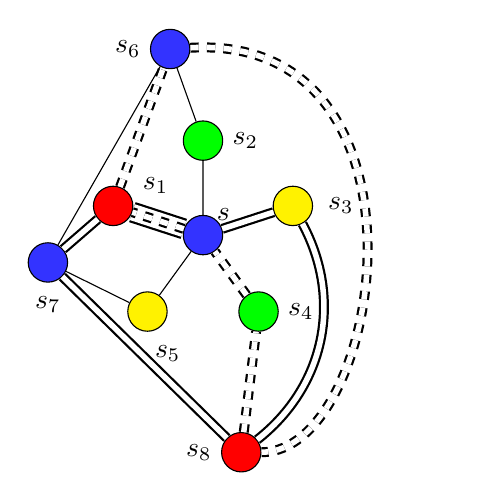
\begin{tikzpicture}[scale=.4,minimum size=5mm,inner sep=0pt]

% Draw center node and adjacent nodes
\foreach \name/\color/\theta in
    {A/yellow/18,B/green/90,C/red/162,D/yellow/234,E/green/306}
  \node[circle,draw,fill=\color] (\name) at (\theta:3) {};
\node[circle,draw,fill=blue!80] (O) at (0,0) {};
\node[above right]     at (O) {$s$};

\node[right,xshift=10pt] at (A) {$s_3$};
\node[right,xshift=8pt]  at (B) {$s_2$};
\node[above right,xshift=8pt]  at (C) {$s_1$};
\node[below right,yshift=-8pt] at (D) {$s_5$};
\node[right,xshift=8pt]  at (E) {$s_4$};

% Draw red-yellow path
\node[circle,draw,fill=blue!80] (X1) at (-170:5) {};
\node[circle,draw,fill=red]  (X2) at (-80:7)  {};

\draw[thick,double distance=2pt] (A) -- (O);
\draw[thick,double distance=6pt] (O) -- (C);
\draw[thick,double distance=2pt] (C) --(X1) -- (X2);
\draw[thick,double distance=2pt,bend right=40] (X2) to (A);

% Draw red-green path
\node[circle,draw,fill=blue!80] (Y1) at (100:6)  {};

\draw[dashed,thick,double distance=2pt] (O) -- (C) -- (Y1);
\draw[dashed,thick,double distance=2pt] 
  (Y1) .. controls (40:10) and (-50:9) .. (X2);
\draw[dashed,thick,double distance=2pt] (X2) -- (E) -- (O);

% Draw adjacent nodes
\draw (X1) -- (D) -- (O) -- (B) -- (Y1) -- (X1);
\node[left,xshift=-8pt] at (Y1) {$s_6$};
\node[below,yshift=-8pt] at (X1) {$s_7$};
\node[left,xshift=-8pt] at (X2) {$s_8$};
\end{tikzpicture}
%\includegraphics[width=\textwidth]{Fig4_12b}
         \captionof{figure}{En échangeant les couleurs, les sommets bleus sont reliés}
         \label{f.five-kempe2-share}
     \end{minipage}


\subsection*{Quelle est la surprise ?}

Le théorème des quatre couleurs est célèbre parce qu'il est facile à énoncer mais extrêmement difficile à démontrer. Il est donc surprenant que la preuve du théorème des cinq couleurs soit élémentaire. La partie la plus intéressante de la démonstration est le théorème~\ref{thm.degree5} (un graphe planaire doit avoir un sommet de degré 5 au maximum), un théorème qui n'a rien à voir avec le coloriage. Au contraire, il résulte simplement du comptage des sommets et des arêtes.

\subsection*{Sources}

Pour le théorème des quatre couleurs, voir \cite{thomas,wiki:four}. La démonstration du théorème des cinq couleurs est basée sur \cite{thebook,wiki:five}.
\cite{eppstein} présente de nombreuses démonstrations de la formule d'Euler. La démonstration erronée du théorème des quatre couleurs par Kempe est décrite dans \cite{sipka}.
